\chapter{Background}\label{kap:background}
\section{Biological Background}\label{sec:biological-background}
\begin{itemize}
      \item \textbf{Genes}: A gene is a basic unit of heredity in a living organism.
            Genes, made up of \ac{DNA}, act as instructions for making molecules called proteins.
            Genes can be gained or lost from bacterial genomes by various mechanisms, affecting the characteristics and abilities of the organism.
      \item \textbf{Genome}: The genome of an organism is the complete set of \ac{DNA}, including all its genes.
            In bacteria, the genome is usually a single circular \ac{DNA} molecule called a chromosome, which contains all the genetic information.
            Bacteria can also contain smaller \ac{DNA} molecules called plasmids, which often carry extra genes.
            Plasmids are also usually circular. The bacterial genome can vary greatly in size and gene content between different species.
      \item \textbf{Bacterial reproduction}: Bacteria reproduce primarily by asexual binary fission, in which a single cell replicates its organelles and genome before dividing into two identical daughter cells.
            This process allows rapid population growth and results genetic uniformity.
\end{itemize}
\subsection{Genetic Diversity}
Despite the clonal reproduction process in bacteria, genetic variation exists.
This diversity stems inter alia from migration, evolutionary selection but also from mutations, gene conversion and horizontal gene transfer.

Mutations are spontaneous changes in the \ac{DNA} sequence, such as single nucleotide polymorphisms, insertions, deletions, and duplications.
These changes can result from errors in \ac{DNA} replication, exposure to environmental factors such as radiation, or the activities of mobile genetic elements.

An important but less frequent mechanism in genetics is gene conversion.
It involves the non-reciprocal transfer of genetic information between homologous sequences, which can result in the replacement of a section of one \ac{DNA} strand with a sequence from a homologous strand.
Gene conversion can occur within a chromosome (allelic conversion) or between different chromosomes (ectopic conversion).

During gene conversion, one segment of \ac{DNA} is replaced by a highly similar (homologous) segment from a different position or \ac{DNA} strand, meaning the two sections end up becoming identical after the process.
Gene conversion often occurs during \ac{DNA} replication or repair.
There, single strands from two similar \ac{DNA} sequences temporarily align.
One strand in the pair breaks, and \ac{DNA} polymerase starts copying the sequence of the other strand to repair the break.
This replaces the corresponding section in the broken strand.

The length of the repaired segment varies and may span a single gene or several genes, depending on the size of the original break and the duration of the strand pairing.
As the broken strand of \ac{DNA} is repaired, the two \ac{DNA} molecules separate.
Unlike traditional `crossing over' in genetic recombination, gene conversion is unidirectional, with one strand acting as the `donor' and overwriting the sequence of the other `recipient' strand.

Horizontal Gene Transfer (\ac{HGT}), also known as lateral gene transfer, is the process of transferring genetic material between different organisms,
bypassing the standard method of genetic inheritance from parent to offspring \cite{HGT_Soucy_2015} \cite{Gen_Molekbio_Schmidt_2023}.
The concept of \ac{HGT} emerged in the late 1940s and initially focused on microorganisms, particularly bacteria and archaea.
In certain cases, the effect was also observed in eukaryotes such as plants \cite{HGT_Eukaryotes_Keeling_2008}.

In bacterial \ac{HGT}, there are several key mechanisms by which it may occur:

\begin{enumerate}
      \item \textbf{Transformation}: This involves the uptake and incorporation of foreign \ac{DNA} or RNA into a cell.
            It occurs naturally in bacteria, but can be induced artificially by exposing cells to heat or electrical pulses.
      \item \textbf{Transduction}: In this process, bacterial \ac{DNA} is transferred from one bacterium to another via a phage.
            Phages are simple entities consisting of genetic material enclosed in a protein shell (capsid) that enables them to attach to the host cell by specifically recognising host proteins.
            The transduction process commences when a phage infects a bacterial cell, turning it into a donor.
            The phage integrates its genome into the bacterial chromosome.
            During excision, part of the bacterial chromosome is accidentally cut out along with the phage \ac{DNA}.
            This excised chromosomal \ac{DNA}, now packaged with the phage \ac{DNA} inside the phage capsule, leaves the donor cell.
            These new phages then infect other cells, transforming them into recipients and transferring the extrachromosomal \ac{DNA} from the original donor.
            One of the best known phages in this context is the lambda phage, famous for its ability to infect E. coli \cite{Gen_Molekbio_Schmidt_2023}.
      \item \textbf{Gene Transfer Agents}: These are virus-like structures found in certain bacteria that facilitate gene transfer.
            They act similarly to bacteriophages, but instead of carrying their own genetic material, GTAs package random fragments of their host's \ac{DNA}.
      \item \textbf{Bacterial Conjugation}: This process uses direct cell-to-cell contact to transfer \ac{DNA} from a donor cell to a recipient cell.
            The most common gene transfer system relies on a piece of \ac{DNA} called an F (fertility) plasmid.
            The donor cell, which carries the F plasmid, forms a pilus, a tube-like structure that extends to make contact with the recipient cell.
            Once contact is made, the F plasmid replicates in the donor cell.
            One of the plasmid strands is then transferred through the pilus into the recipient cell.
            If the plasmid integrates into the genome, it is likely that neighbouring genes will also be transferred.
            It is important to note that this process is usually unidirectional,
            i.e. genetic material can be transferred from the donor to the recipient, but not vice versa.
            After the transfer, the recipient cell synthesises a complementary strand to the incoming single-stranded \ac{DNA},
            forming a complete plasmid.
            This genetic material can be incorporated into the recipient's genome or exist as an independent plasmid within the cell.
\end{enumerate}

These events may lead to genetic changes that can, but do not always, result in different phenotypes.
In some species, such as Buchnera aphidicola, genetic variation accumulates mainly through point mutations.
This characteristic, together with its very small genome size of 500kb and only 350-590 genes \cite{Buchnera},
makes Buchnera aphidicola of particular interest for the simulation part of this work.

In other species, such as \ac{MRSA}, the effect of \ac{HGT} is crucial.
This strain is thought to have acquired resistance genes horizontally from animal-associated bacteria.
Once a strain acquires resistance, it multiplies and evolves as it becomes more likely to spread between patients and healthcare facilities.
This phenomenon is not limited to specific bacterial lineages, but occurs across different strains and sometimes even Kingdoms \cite{HGT_Kingdom_Richards_2011} leading to the emergence of diverse populations.
In contrast to species with a strong clonal or \ac{HGT} effect, organisms such as Streptococcus pneumoniae and Neisseria meningitidis exhibit high rates of homologous recombination \cite{Panstripe_Tonkin_Hill_2023} \cite{HGT_Burmeister_2015}.

\section{Simulation Background}\label{sec:simulation-background}
The latter described simulation algorithm uses a concept called the pangenome.
The pangenome is the set of all genes carried by all individuals in a population, reflecting the genetic variation and potential for adaptation.
It can be divided into two main parts:

\begin{enumerate}
      \item \textbf{Core Genome} $G_c$: The core genome consists of genes present in every individual of the population.
            These genes are often essential for survival and reproduction and known to be highly conserved.
      \item \textbf{Dispensable / Individual Genome} $G_i$: These are genes that are not present in all individuals but may confer selective advantages in certain environments or conditions.
\end{enumerate}

The concept of a pangenome was first proposed and analysed for pathogenic strains of Streptococcus agalactiae by Tettelin et al. in 2005 \cite{Tettelin_2005}.
Their analysis showed that approximately 80\% of the genes in a single S. agalactiae genome are shared by all individuals and are therefore part of $G_c$.
However, each fully sequenced genome contains unique genes that are not found in other individuals.
This aligns with  the distributed genome hypothesis, proposed by Ehrlich et al.
in 2005 \cite{Ehrlich_2010} stating that no single organism possesses the entire set of genes of its species.
Species with a small dispensable genome are typically referred to as `closed', while those with a highly variable dispensable genome are referred to as `open'.

\subsection{Wright-Fisher Model}
The Wright-Fisher model is a key concept in population genetics and is used to describe the evolution of the genetic composition of a population over time \cite{WF_Model_Messer_2016}.
It is particularly suitable for prokaryotes, such as bacteria and archaea, as its concepts are centred on asexual reproduction.

The model assumes a constant population size and that the population evolves through discrete, non-overlapping generations.
This means that each generation is distinct from the previous one.
This size, denoted $N_e$, is the effective number of individuals able to contribute to the next generation rather than the total number of individuals.
For sexually reproducing organisms, $N_e$ is strongly influenced by location, physical distance, but also by mating and social aspects \cite{Human_Popgen_Lohmueller_2021}.

For example, the effective population size for humans is estimated to be 10,000, despite a census population size of 8.1 billion ($8.1 \times 10^9$).
Similarly, for Prochlorococcus, a marine cyanobacterium responsible for 10\% of global oxygen production, $N_e$ is set to a relatively small $1.68 \times 10^7$ \cite{Prochlorococcus_Chen_2021},
although the actual population size is around $3 \times 10^{27}$ \cite{Prochlorococcus_Flombaum_2013}.

\begin{figure}[h]
      \centering
      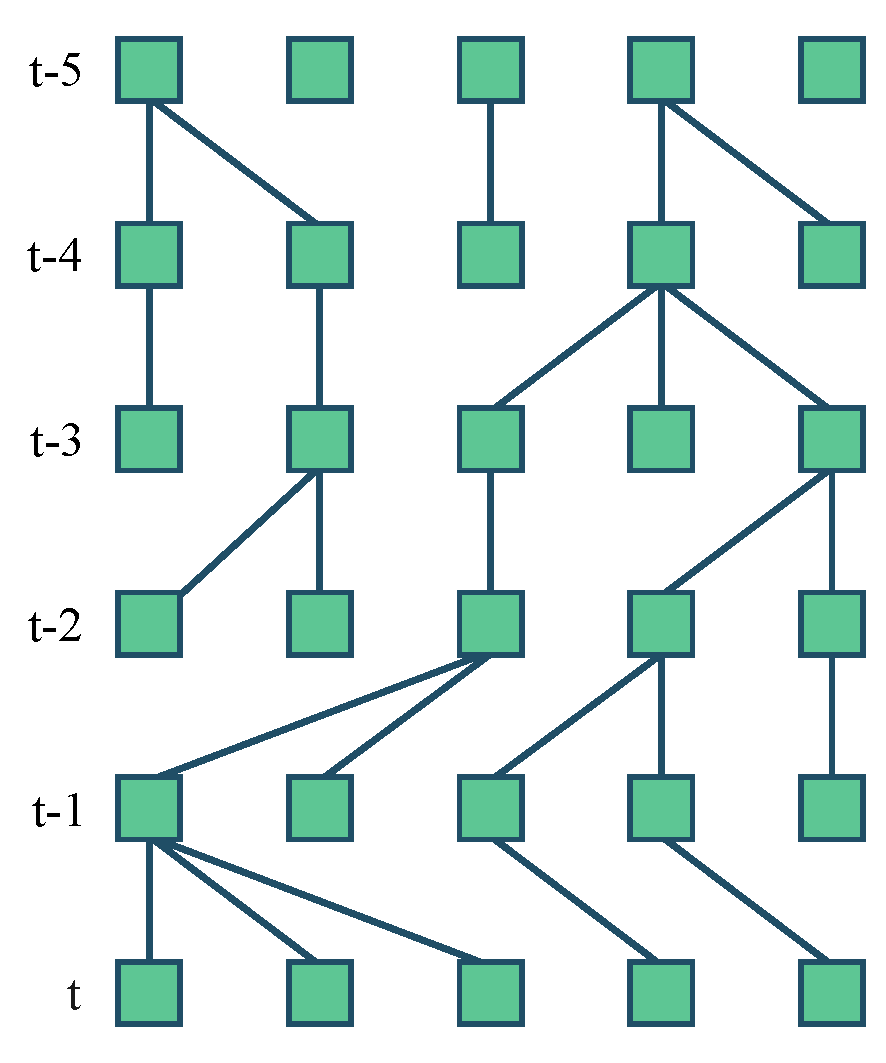
\includegraphics[width=0.4\textwidth]{figures/wf.pdf}
      \caption[Wright-Fischer model.]{Wright-Fischer model with 5 generations. Every individual chooses one parent at random.}
      \label{fig:wright-fisher}
\end{figure}

The Wright-Fisher model is best described backwards in time.
Assuming neutral clonal (i.e. asexual) reproduction, with no selection, mutation or migration, each individual of generation $t$ chooses a single parent from the previous generation $t-1$.
This means that several individuals can have the same parent, and each parent has an equal chance of survival and reproduction, as seen in figure \ref{fig:wright-fisher}.
If two individuals have a common ancestor, their lineages are said to coalesce.

The process of selecting parents in each generation follows a uniform random pattern.
Therefore, the probability of a given individual being selected as a parent is $1/N$ and, conversely, the probability of that individual not being selected is $1-1/N$.
Modelling this selection forwards in time, the number of offspring can be represented as a binomial distribution $X \sim B(n=N, p=1/N)$.
For large populations ($N >> 20$), the number of offspring an individual has follows a Poisson distribution.
This is due to the Poisson limit theorem, which allows the underlying binomial distribution to be approximated by the Poisson distribution for sufficiently large $N$:

\begin{equation}
      P[X=k] = \lim _{n\to \infty }{n \choose k}p_{n}^{k}(1-p_{n})^{n-k}=e^{-\lambda }{\frac {\lambda ^{k}}{k!}}
\end{equation}

The average number an individual is chosen as a parent is $E[X] = n \cdot p = 1$.
As the expected value of a Poisson distribution is:
\begin{equation}
      E[X] = \sum^\infty_{k=0} k \cdot e^{-\lambda }{\frac {\lambda ^{k}}{k!}} = \lambda
\end{equation}
we know that under this model, the number of offspring of an individual has, is approximately Poisson distributed with $\lambda = 1$.

\subsection{Kingman coalescent}\label{subsec:kingman}
The Kingman coalescent is a stochastic process that models the genealogical history of a sample of genes from a population and is closely related to the Wright-Fisher model.
It is also known as the standard neutral coalescent model \cite{Human_Popgen_Lohmueller_2021}.

By examining all possible events of the (haploid) Wright-Fisher model in the immediate ancestry of a generation, Kingman found that a single coalescent event between two individuals is the most probable event.
Averaging over multiple generations and considering all possible combination if individuals, the probability of a coalescent event is then given by

\begin{equation}
      p_\text{c} = \binom{n}{2} \frac{\sigma^2}{N} + O\left(\frac{1}{N^2}\right)
\end{equation}

where $n$ is the number of samples, $\sigma^2$ is the variance of the number of offspring of a single individual \cite{Kingman_1982}.
The binomial coefficient $\binom{n}{2}$ describes the number of possible lineage pairs.
This equation assumes large populations where the exact probability is approximated by the first term;
the term $O(1/N^2)$ represents the remaining coalescence of two or more lineages. The largest element of this power series expansion is proportional to $1/N^2$.
As $N \to \infty$, the additional terms become negligible, leaving the first term alone.

As time is rescaled by the population size $N$, and as $N$ approaches infinity, the time to \ac{MRCA} of two samples converges to an exponential distribution $f(t) = e^{-t}$.
The rate of coalescence between two lineages on the new timescale is thus 1, meaning that in a population of $n$ individuals with $n(n-1)/2$ possible pairs, the rate of coalescence is $n(n-1)/2$.

If this model is simulated backwards in time and $n$ lineages remain, the exponential waiting time is calculated with a rate of $n(n-1)/2$.
This rate corresponds to the number of possible pairs of lineages that can coalesce, as each pair has a chance of coalescing into a single line.
At the time of coalescence, two lines are randomly selected from the remaining $n$ lines and merged into one.
The simulation continues until only one line remains, the \ac{MRCA}.

\subsection{Gene Frequency Spectrum}
The \ac{GFS} is a method of summarising genetic diversity within a population by classifying genes according to their frequency among individuals.
It is similar to the allele frequency spectrum.
Taking the number of genes present in exactly $k$ different individuals within a sample of size $n$ gives the gene frequency class $G_k^{(n)}$.

For instance, in a population of 100 individuals, the gene frequency class of $G_5^{(100)}$ represents the number of genes found in exactly 5 of those individuals.

For random trees without horizontal gene transfer the expected value $E[G_k]$ is given by
\begin{equation}
      \mathbb{E}[G_k] = \frac{\theta}{k(n - 1 + \rho)(n - k + \rho)}
\end{equation}
which gives us, depending on $\theta$ and $\rho$, a distinct L or U shape.
As can be seen in figure \ref{fig:typical-gfs}, higher $\rho$ cause gene loss events to dominate over gene gains, resulting in an L-shape with few high-frequency genes.
\begin{figure}[h]
      \centering
      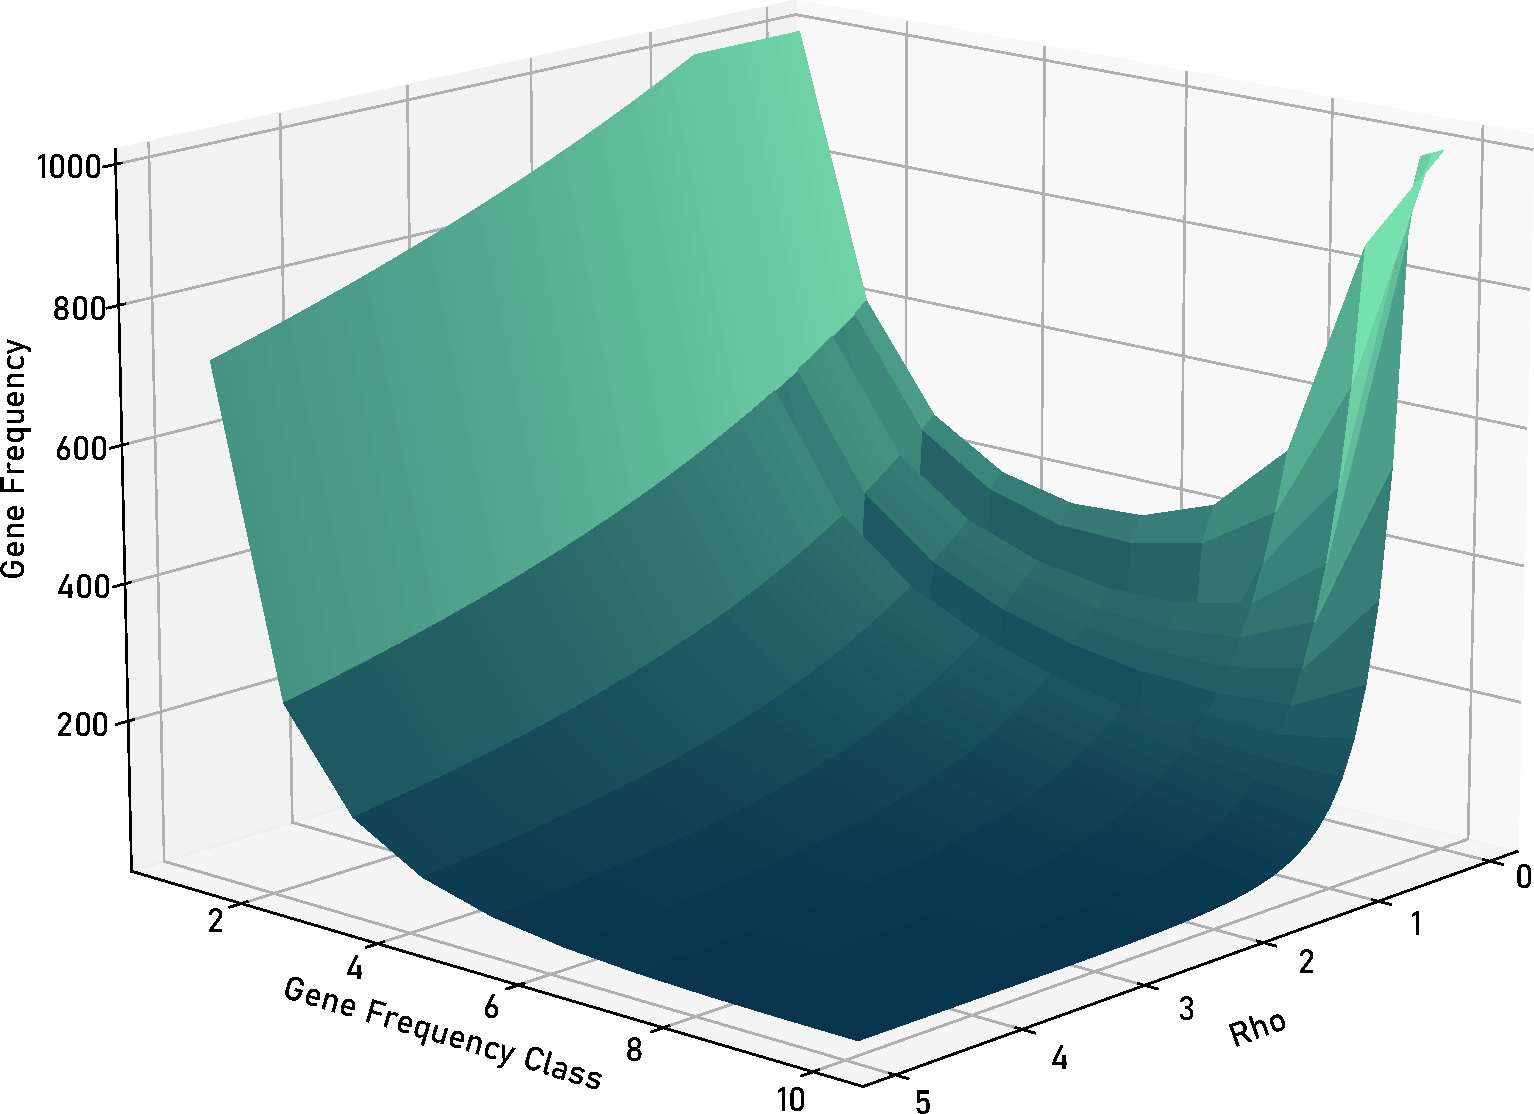
\includegraphics[width=0.7\textwidth]{figures/gfs_ratio.pdf}
      \caption[Expected Gene Frequency Spectrum.]{Expected Gene Frequency Spectrum for different gene loss rates $\rho$ at fixed gene gain $\theta = 1000$ for 10 samples.}
      \label{fig:egfs}
\end{figure}

If, on the other hand \ac{HGT} is present, Baumdicker et al. \cite{Baumdicker_2014} estimated the expected \ac{GFS} for large populations $n$ and $\rho > 0, \theta > 0, \gamma \geq 0$  to be
\begin{equation}
      \mathbb{E}\left[ G_k^{(n)} \right] = \frac{\theta}{k} \frac{(n)_k\downarrow}{(n-1+\rho)_k\downarrow} \left( 1 + \sum_{m=1}^{\infty} \frac{(k)_m\uparrow \gamma^m}{(n+\rho)_m\uparrow m!} \right)
\end{equation}
with $(a)_{b\uparrow} := a (a+1) \cdots (a+b-1)$ and $(a)_{b\downarrow} := a (a-1) \cdots (a-b+1)$.
In other words, genes appear with higher frequency, leading to a closed genome.

\newpage
\subsection{Infinitely Many Genes Model}
The \ac{IMG} model \cite{Baumdicker_2010} \cite{Baumdicker_2012} is the cornerstone of this work.
It allows us to place gene gain and loss events along the ancestral lineages of individuals on the Kingman coalescent.

In this model, a gene can only be gained once, but has the potential to be lost multiple times independently on different branches.
In addition, gene gain is exclusively associated with mutation rather than horizontal gene transfer.

To keep this model simple, the core genes $G_c$, which are essential for survival and reproduction, are ignored.

Beyond $G_c$, there exists an infinite pool of genes $I$ with $G_c \cap I = \varnothing$.
The genome of individual $i$ in the sample, $1 \leq i \leq N$, contains the set of genes $G_i \subseteq I$ that are not necessary for the individuals to survive.

\begin{enumerate}
      \item \textbf{Gene Gain} There is a probability $\mu$ before reproduction that an individual will acquire a new gene from the environment,
            which is assumed to have never been present in the population's gene pool before.
      \item \textbf{Gene Loss} Each gene in the dispensable genome $G_i$ of an individual $i$ has a probability $v$ of being lost before the reproduction event.
\end{enumerate}
As we are working with the Kingman coalescent, time is measured in units of $N_e$ instead of generations.
Thus, the mutation rates $\mu$ and $v$  are rescales in line with the genealogies so that $\theta = \lim_{N\rightarrow\infty} N\cdot \mu$ and $\rho = \lim_{N\rightarrow\infty} N\cdot v$

Following Baumdicker et al. \cite{Baumdicker_2010} we therefore get the average number of genes, in the dispensable genome, by the formula:

\begin{equation}
      A = \frac{1}{n} \sum_{i=1}^{n} |G_i|
\end{equation}

For $A$ as defined above, the expected value is given by:

\begin{equation}
      \mathbb{E}[A] = \frac{\theta}{\rho}
\end{equation}


where $\theta$ and $\rho$ are the gene gain and loss rates, respectively.


The \ac{IMG} model differs from the traditional \ac{FMG} model, in which genes can be repeatedly gained and lost within evolutionary lineages.
In the \ac{IMG} framework, we assume an infinite pool of potential genes, whereas the \ac{FMG} model, on the other hand, assumes a finite set of $M$ possible gene types.
Each gene gained is selected from this pool, so it is possible for the same gene to be gained several times during the evolutionary process.
The overall rate at which genes are gained is $\theta=a \cdot M$, where a represents the gain rate of individual gene type.
The \ac{IMG} model can be seen as a limiting case of the FMG model, where the size of the gene pool $M$ approaches infinity as the rate of gain of a particular gene $a$ approaches zero, while the overall rate of gain $\theta$ remains constant.

Both models treat genes, gene gains and gene losses as independent entities / events, ignoring any positional effects or genomic order, such as the simultaneous loss of entire genomic regions containing multiple genes.
Furthermore, both models assume constant rates of gene gain and loss over time, despite known variations in these rates.

In this model, Horizontal Gene Transfer events between any two individuals $i$ and $j$ occur at a rate of $\gamma / N$ for each gene $u \in G^N_i(t)$ in the genome of individual $i$ at time $t$.
During such an event, the gene $u$ is duplicated from the donor $i$ to the recipient $j$, resulting in the addition of $u$ to $G^N_j(t)$, the gene set of $j$, while maintaining $u$ in $G^N_i(t)$.

If the recipient $j$ already has the gene $u$, the transfer event has no effect because the model excludes paralogous gene creation.
While it is possible for bacteria to transfer multiple genes at once, this effect is neglected in this work as and each \ac{HGT} event is responsible for only one gene.

\subsection{msprime and tskit}
\textit{msprime} is a fast and flexible coalescent-based simulator.
It can efficiently simulate the genealogies (ancestral recombination graphs) of individuals under different evolutionary models and
is based on \textit{tskit} which provides a compact data format for storing and manipulating tree sequences \cite{Msprime_Kelleher_2016} \cite{Msprime_Baumdicker_2022}.
Both provide a python interface with C backbone.
In the following work we will extend and use the \textit{msprime} and \textit{tskit} software packages.


To ensure clarity and precision, we provide a summary of their key terms and concepts:
\begin{itemize}
      \item \textbf{Tree}: Refers to a genealogical tree outlining the relationships between a collection of genomes at a given chromosomal location.
      \item \textbf{Node}: A node is a branching point in a tree at a given time.
            At this node, several segments have come together. Non-branching nodes can exist.
      \item \textbf{Segment}: A segment represents a section of the genome.
            Each segment contains a left and right position indicating the boundaries within the genome, a reference node, and a pointer to the next and previous segments in the chain.
            Together, these segments form a chain that can (but are not required to) cover the entire genome.
      \item \textbf{Lineage}: If the head (left-most) segment  of a segment chain is present in our population, this chain is considered a lineage.
      \item \textbf{Edge}: An edge is defined as a tuple marking a parent-child relationship between nodes across the boundaries (left, right) of a given segment.
      \item \textbf{Site}: A site is a unique position on the genome, associated with an allele.
      \item \textbf{Mutation}: This term refers to a change in state at a site that occurs above a particular node.
            Each mutation is linked to a specific site and node and has a defined derived state.
\end{itemize}

At the heart of \textit{msprime} is the so-called `hudson simulation loop', which iteratively models events that alter ancestral relationships.
Initially, a separate lineage is created for each individual.
Each lineage each consist of a segment spanning the entire genome and is associated with a unique (leaf) node.
The head of each lineage is referenced in the population, a hashmap for quick access.
The simulation loop continues as long as there are multiple lineages and the simulation time is less than a specified end time.


\begin{enumerate}
      \item \textbf{Calculate event times}: As first step, the waiting time for each of the next possible events is calculated.
            These values range from 0 to positive infinity and follow an exponential distribution based on the input parameters.
            Gene gains are initialised with a rate of $\theta$, losses with a rate of $\rho$, and gene conversion events with $\kappa$.
            It should be noted that $\rho$ and $\kappa$ are parameters that are relative to the total number of sites $s$.
      \item \textbf{Determine next event}: The function identifies the next event based on the minimum of the calculated times (\mintinline{python}{min_time}).
      \item \textbf{Execute event}:
            \begin{itemize}
                  \item Gene conversion (`GCI', `GCL'): A small sub-segment (alpha) is cut from a randomly selected segment.
                        This copied sub-segment is inserted into the population and forms a new, independent lineage.
                  \item Recombination (`REC'): A breakpoint of a random line is selected, and a segment is split at this position.
                        By removing the link in the segment chain and adding the new orphaned chain to the population, this segment chain is treated as a separate lineage in the rest of the simulation.
                  \item Common Ancestor Event (`CA'): Two random lines are selected.
                        A new node is inserted in the tree to represent this common ancestor, where the two lineages are merged.
                        Edges are added that span the width of overlapping segments of both lineages.
                        These edges will later be used for mutation simulation.
            \end{itemize}
      \item \textbf{Table building} After the simulation, the resulting tree is passed to the \textit{tskit} library which uses a series of linked tables,

      \item \textbf{Mutation simulation}: If desired, mutations can be placed along the edge using different models.
\end{enumerate}
\newpage
\begin{figure}[h]
      \centering
      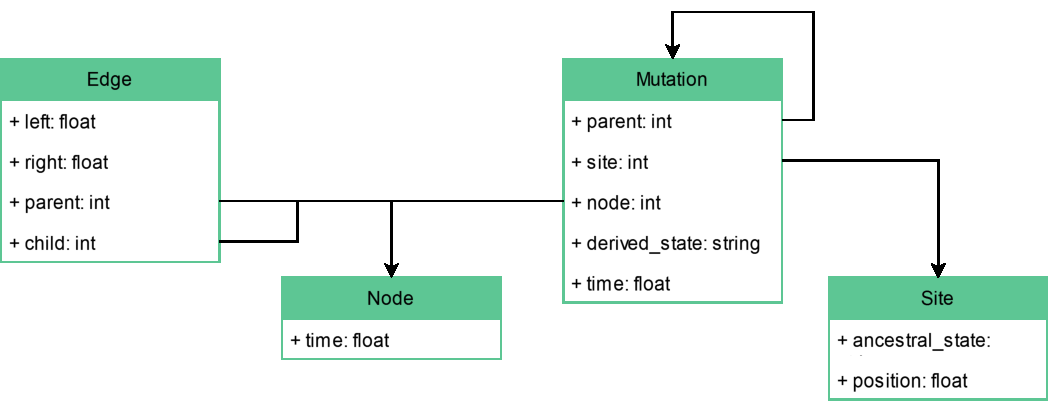
\includegraphics[width=\textwidth]{figures/tables_uml.pdf}
      \caption{Relation of the tables managed by \textit{tskit}.}
      \label{fig:tables-uml}
\end{figure}

The tables created during the simulation store the underlying data and are managed by \textit{tskit}.
Figure \ref{fig:tables-uml} shows the 4 main tables and omits some columns for simplicity.
It is important to note that each row in a table has an indirect identifier based on its position, which can be references in other tables.

As nodes represent branching points in the tree where several segments have come together, the Node Table stores the time of these points.
The Edge Table describes parent-child relationships between nodes over specific genomic intervals, with the left column denoting the inclusive start position and the right column denoting the exclusive end position.
The Mutation table records mutation details within the genome:
\begin{itemize}
      \item Parent: Identifier for the parent mutation.
      \item Site: Identifier of the mutation site.
      \item Node: Identifier for the node below which the mutation is observed.
      \item Derived State: The allelic state resulting from the mutation.
      \item Time: The time of occurrence.
\end{itemize}

The Site Table maps locations on the genome where allelic states are observed:
\begin{itemize}
      \item Position: The exact genomic location. As we are using a discrete genome, the location must fall on an integer, although rational numbers are supported.
      \item Ancestral state: The allelic state at the root of the tree, before any mutations.
\end{itemize}
To store a complete tree structure, only the edge and Node Tables are required.
If mutations are added, both an additional Mutation table and a Site Table must be added.
The sum of all tables is a \mintinline{python}{TableCollection} to which the \textit{tskit} interface provides indirect access via \mintinline{python}{RowObjects} or direct access to the underlying \textit{numpy} arrays.